\documentclass{beamer}\usepackage[]{graphicx}\usepackage[]{color}
%% maxwidth is the original width if it is less than linewidth
%% otherwise use linewidth (to make sure the graphics do not exceed the margin)
\makeatletter
\def\maxwidth{ %
  \ifdim\Gin@nat@width>\linewidth
    \linewidth
  \else
    \Gin@nat@width
  \fi
}
\makeatother

\definecolor{fgcolor}{rgb}{0.345, 0.345, 0.345}
\newcommand{\hlnum}[1]{\textcolor[rgb]{0.686,0.059,0.569}{#1}}%
\newcommand{\hlstr}[1]{\textcolor[rgb]{0.192,0.494,0.8}{#1}}%
\newcommand{\hlcom}[1]{\textcolor[rgb]{0.678,0.584,0.686}{\textit{#1}}}%
\newcommand{\hlopt}[1]{\textcolor[rgb]{0,0,0}{#1}}%
\newcommand{\hlstd}[1]{\textcolor[rgb]{0.345,0.345,0.345}{#1}}%
\newcommand{\hlkwa}[1]{\textcolor[rgb]{0.161,0.373,0.58}{\textbf{#1}}}%
\newcommand{\hlkwb}[1]{\textcolor[rgb]{0.69,0.353,0.396}{#1}}%
\newcommand{\hlkwc}[1]{\textcolor[rgb]{0.333,0.667,0.333}{#1}}%
\newcommand{\hlkwd}[1]{\textcolor[rgb]{0.737,0.353,0.396}{\textbf{#1}}}%

\usepackage{framed}
\makeatletter
\newenvironment{kframe}{%
 \def\at@end@of@kframe{}%
 \ifinner\ifhmode%
  \def\at@end@of@kframe{\end{minipage}}%
  \begin{minipage}{\columnwidth}%
 \fi\fi%
 \def\FrameCommand##1{\hskip\@totalleftmargin \hskip-\fboxsep
 \colorbox{shadecolor}{##1}\hskip-\fboxsep
     % There is no \\@totalrightmargin, so:
     \hskip-\linewidth \hskip-\@totalleftmargin \hskip\columnwidth}%
 \MakeFramed {\advance\hsize-\width
   \@totalleftmargin\z@ \linewidth\hsize
   \@setminipage}}%
 {\par\unskip\endMakeFramed%
 \at@end@of@kframe}
\makeatother

\definecolor{shadecolor}{rgb}{.97, .97, .97}
\definecolor{messagecolor}{rgb}{0, 0, 0}
\definecolor{warningcolor}{rgb}{1, 0, 1}
\definecolor{errorcolor}{rgb}{1, 0, 0}
\newenvironment{knitrout}{}{} % an empty environment to be redefined in TeX

\usepackage{alltt}
\usepackage[utf8]{inputenc}
\usepackage[T1]{fontenc}
\usepackage[brazil]{babel}
\usepackage{graphicx}
\usepackage{verbatim}
\usepackage{alltt}
\usepackage{here}
\usepackage{xcolor}
\usepackage{fancyhdr}
\usepackage{setspace}
\usepackage{indentfirst}
\usepackage{multirow}
\usepackage{makeidx}
\usepackage{wrapfig}
\usepackage[all]{xy}
\usepackage{fancybox}
\usepackage{rotating}
\usepackage{eso-pic}
\usepackage{dcolumn}
\usepackage{color}
\usepackage{lscape}
\usepackage{subfigure}
\usepackage{scalefnt}

\newcommand{\ds}{\displaystyle}

\usetheme{CambridgeUS}

\definecolor{ESALQ}{RGB}{50,93,61}
\definecolor{DarkSeaGreen}{RGB}{143,188,143}
\definecolor{PaleGreen}{RGB}{84,139,84}
\setbeamercolor{frametitle}{fg=black,bg=DarkSeaGreen}
\setbeamercolor{structure}{fg=ESALQ}
\setbeamercolor{palette primary}{fg=ESALQ}
\setbeamercolor{palette secondary}{fg=ESALQ}
\setbeamercolor{palette tertiary}{bg=ESALQ}
\setbeamercolor{title}{fg=black,bg=DarkSeaGreen}
\setbeamercolor{block title}{fg=black,bg=DarkSeaGreen}
\setbeamercolor{block title alerted}{bg=DarkSeaGreen}
\makeindex

\usepackage{xspace}
\providecommand{\eg}{\textit{e.g.}\xspace}
\providecommand{\ie}{\textit{i.e.}\xspace}
\providecommand{\R}{\textbf{R}\xspace}
\providecommand{\emacs}{\textbf{Emacs}\xspace}
\providecommand{\knitr}{\textbf{knitr}\xspace}
\providecommand{\rstudio}{\textbf{RStudio}\xspace}

%% Fontes para codigo
\usepackage[scaled]{beramono} % truetype: Bistream Vera Sans Mono
%\usepackage{inconsolata}

\title[Introdução ao $\LaTeX$]{Introdução ao $\LaTeX$}
\author[]{\small Bruna Gabriela Wendpap \\
  Djair Durand Ramalho Frade \\
  Fernando de Pol Mayer \\
  Luiz Ricardo Nakamura \\
  Maria Cristina Martins \\
  Thiago de Paula Oliveira \\
  Thiago Gentil Ramires \\
  Profa. responsável: Dra. Roseli Aparecida Leandro
}
\institute[ESALQ/USP]{Universidade de São Paulo (USP) \\
  Escola Superior de Agricultura ``Luiz de Queiroz" (ESALQ)}
\date[]{04 de Outubro, 2013}

 \AtBeginSection[]
 {
   \begin{frame}
     \frametitle{Plano de aula}
     \tableofcontents[currentsection]
   \end{frame}
 }

 \AtBeginSubsection[]
 {
   \begin{frame}
     \frametitle{Plano de aula}
     \tableofcontents[currentsection,currentsubsection]
   \end{frame}
 }
\IfFileExists{upquote.sty}{\usepackage{upquote}}{}

\begin{document}
\pgfdeclareimage[height=1.4cm]{logo}{esalq}
\logo{\pgfuseimage{logo}}
\frame{\titlepage}




\begin{frame}{Sumário}
\tableofcontents
\end{frame}

\section{Introdução}

\begin{frame}{Introdução}
Teste
\end{frame}

\section{Configuração}

\begin{frame}[fragile]{Configuração}
  \begin{itemize}
  \item O \knitr pode ser utilizado em qualquer editor de texto, mas
    alguns facilitadores são
    \begin{itemize}
    \item \emacs com ESS
    \item LyX
    \item \rstudio
    \end{itemize}
  \item A primeira coisa a fazer no \R é instalar os pacotes necessário:
\begin{knitrout}\footnotesize
\definecolor{shadecolor}{rgb}{0.969, 0.969, 0.969}\color{fgcolor}\begin{kframe}
\begin{alltt}
\hlkwd{install.packages}\hlstd{(}\hlkwd{c}\hlstd{(}\hlstr{"knitr"}\hlstd{,} \hlstr{"xtable"}\hlstd{),} \hlkwc{dependencies} \hlstd{=} \hlnum{TRUE}\hlstd{)}
\end{alltt}
\end{kframe}
\end{knitrout}

  \end{itemize}
\end{frame}

\begin{frame}[fragile]{Configuração}
A ideia é fazer a seguinte sequência:
\begin{enumerate}
\item Criar um arquivo com a extensão \texttt{.Rnw}
\item Inserir o preâmbulo tradicional do \LaTeX{}, texto e código
\item Compilar o arquivo com a função \texttt{knit()} $\rightarrow$ vai
  gerar um arquivo \texttt{.tex}
\item Compilar o arquivo \texttt{.tex} no \TeX{}Maker (ou outros)
  $\rightarrow$ gera o arquivo \texttt{.pdf}
\end{enumerate}
\end{frame}

\begin{frame}[fragile]{Configuração}
Expressões do \R são inseridas normalmente dentro de um ambiente especial
no arquivo \texttt{.Rnw}:
\begin{verbatim}
<<>>=
...
@
\end{verbatim}
\begin{itemize}
\item Toda expressão do \R que estiver dentro deste \textbf{chunk} será
interpretada quando coompilada pelo \knitr, gerando a saída, gráficos,
etc.
\item Para inserir resultados no meio do texto (\textit{inline}) use
  \verb|\Sexpr{}|
\end{itemize}
\end{frame}

\begin{frame}[fragile]{Configuração}
  \begin{block}{Um exemplo mínimo:}
    \footnotesize
\begin{verbatim}
\documentclass{article}
\usepackage[utf8]{inputenc}
\usepackage[T1]{fontenc}
\usepackage[brazil]{babel}
\usepackage[margin=2.5cm]{geometry}

\begin{document}

Definindo a variável aleatória $X$ com distribuição Normal padrão, ou
seja, $X \sim \textrm{N}(0,1)$
<<>>=
set.seed(1)
(x <- rnorm(10))
@
A média desta variável aleatória é %\%Sexpr{mean(x)}. O primeiro
valor é $X_i = %\%Sexpr{x[1]}$.

\end{document}
\end{verbatim}
\end{block}
\end{frame}

\begin{frame}[fragile]{Configuração}
No \rstudio, altere as opções para deixar o \knitr como padrão
\begin{figure}[h]
  \centering
  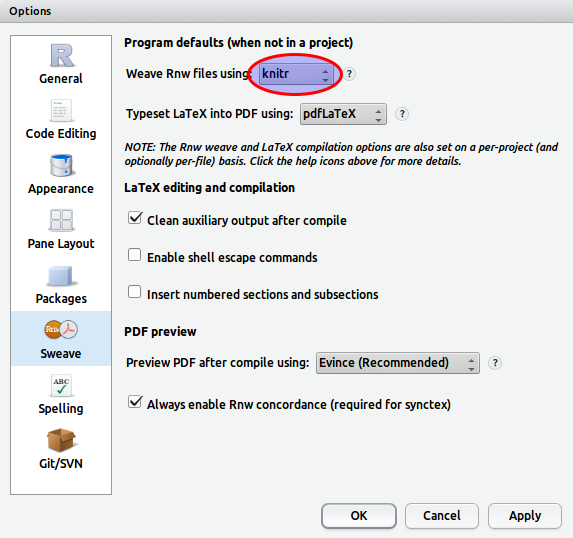
\includegraphics[height=.7\textheight]{RStudio_sweave.png}
\end{figure}
\end{frame}

\begin{frame}[fragile]{Configuração}
Com isso, o botão \textbf{Compile PDF}:
\begin{itemize}
\item Compila o arquivo \texttt{.Rnw} com o \knitr
\item Compila o arquivo \texttt{.tex} resultante com o PDF\LaTeX
\item Abre o PDF no editor padrão
\end{itemize}
\begin{block}{}
  Tudo isso é feito em um ambiente separado da sua área de trabalho
  original, para não haver confusão com objetos gerados
\end{block}
\end{frame}

\section{Opções}

\begin{frame}[fragile]{Opções}
  \begin{itemize}
  \item \textbf{Opções específicas}: são opções definidas para cada
    \textit{chunk} de código, especificadas entre \verb|<<| e \verb|>>|
  \item \textbf{Opções globais}: são opções definidas para todos os
    \textit{chunks} do documento, especificadas pela função do \knitr
\begin{knitrout}\footnotesize
\definecolor{shadecolor}{rgb}{0.969, 0.969, 0.969}\color{fgcolor}\begin{kframe}
\begin{alltt}
\hlstd{opts_chunk}\hlopt{$}\hlkwd{set}\hlstd{()}
\end{alltt}
\end{kframe}
\end{knitrout}

Ainda assim, é possível especificar opções para \textit{chunks} individuais!
\end{itemize}
\end{frame}

\begin{frame}[fragile]{Opções}
  A lista completa de opções está em
  \small\url{http://yihui.name/knitr/options}\normalsize \vspace{2em}
  Algumas opções gerais (* indica o padrão):
  \begin{itemize}
  \item \texttt{eval}: \texttt{TRUE}*, \texttt{FALSE}, ou
    \texttt{c(1,3,4)} ou \texttt{-(4:6)}. Se o código deve ser interpretado
    ou não. Podem ser especificadas apenas linhas.
  \item \texttt{echo}: \texttt{TRUE}*, \texttt{FALSE}, ou
    \texttt{c(1,3,4)} ou \texttt{-(4:6)}. Se deve mostrar ou não o
    código ou pedaços dele. O resultado sempre aparece. (Diferente de
    \texttt{eval}, porque sempre será interpretado).
  \item \texttt{include}: \texttt{TRUE}*, \texttt{FALSE}. Se deve incluir ou não o
    código no documento final. Útil por exemplo para fazer cálculos
    auxiliares que não precisam ser mostrados no documento.
  \end{itemize}
\end{frame}

\begin{frame}[fragile]{Opções}
Algumas considerações sobre as opções:
\begin{itemize}
\item Cada chunk pode ter um nome, por exemplo
\begin{verbatim}
<<bloco1>>=
@
\end{verbatim}
que será útil posteriormente para dar nomes à figuras e extração de
código.
\item Evite usar espaços e pontos nos nomes dos chunks (use \verb|-| e
  \verb|_|).
\item As opções em \verb|<<>>=| devem estar sempre na \textbf{mesma linha}
\item \textbf{Todas} as opções devem ser expressões válidas do \R
  \begin{itemize}
  \item Caracteres entre aspas
  \item Valores lógicos: \texttt{TRUE} ou \texttt{FALSE}
  \end{itemize}
\end{itemize}
\end{frame}

\begin{frame}[fragile]{Opções}
  \begin{alertblock}{Exercício}
    \begin{itemize}
    \item Insira mais 3 chunks no seu arquivo, cada um com pelo menos 3
      linhas de código do \R
    \item Teste as opções \texttt{eval}, \texttt{echo}, e
      \texttt{include} em cada uma delas
    \end{itemize}
  \end{alertblock}
\end{frame}

\begin{frame}[fragile]{Opções}
Opções para decoração de código:
\begin{itemize}
\item \texttt{prompt}: \texttt{TRUE} ou \texttt{FALSE}*. Se deve
  ou não inserir o \textit{prompt} (\verb|>|) do \R no início de cada
  linha.
\item \texttt{comment}: \verb|"##"|* ou \texttt{NA}. Se deve ou não
  comentar a saída dos comandos
\item \texttt{highlight}: \texttt{TRUE}* ou \texttt{FALSE}. Se deve
  colorir os códigos.
\item \texttt{size}: \verb|"normalsize"| ou qualquer tamanho de fonte do
  \LaTeX{} (\verb|"small"|, \verb|"footnotesize"|, $\ldots$)
\item \texttt{tidy}: \texttt{TRUE}* ou \texttt{FALSE}. Se o código deve
  ser formatado para um padrão geral pré-definido.
\end{itemize}
\end{frame}

\begin{frame}[fragile]{Opções}
  \begin{alertblock}{Exercício}
    \begin{itemize}
    \item Altere estas opções em alguns chunks e veja o resultado
    \item Em especial escreve esse código dentro de dois chunks separados
\begin{knitrout}\footnotesize
\definecolor{shadecolor}{rgb}{0.969, 0.969, 0.969}\color{fgcolor}\begin{kframe}
\begin{alltt}
\hlkwd{rnorm}\hlstd{(}\hlnum{10}\hlstd{,}
      \hlnum{10}\hlstd{,} \hlnum{5}\hlstd{)}
\end{alltt}
\end{kframe}
\end{knitrout}

cada um com \texttt{tidy=TRUE} e \texttt{tidy=FALSE}.
    \end{itemize}
  \end{alertblock}
\end{frame}

\begin{frame}[fragile]{Opções globais}
Para definir um padrão para todos os chunks globalmente, podemos
especificar logo no início do documento as opções que queremos. Por
exemplo:
\begin{verbatim}
<<setup, include=FALSE, cache=FALSE, tidy=FALSE>>=
# Minhas configurações globais para os chunks
opts_chunk$set(size = "small",
               prompt = FALSE,
               comment = NA,
               tidy = FALSE,
               cache = TRUE)
@
\end{verbatim}
\end{frame}

\begin{frame}[fragile]{Opções}
  O \texttt{cache} (\texttt{TRUE}*/\texttt{FALSE}):
  \begin{itemize}
  \item Armazena os resultados dos chunks em disco
    \begin{itemize}
    \item Cria um diretório \verb|cache|
    \end{itemize}
  \item Esse resultado será reaproveitado nas próximas compilações,
    portanto um chunk em cache não será interpretado novamente
  \item Muito útil para documentos muito longos ou com comandos
    demorados ou bases de dados grandes
  \end{itemize}
\end{frame}

\section{Tabelas}

\begin{frame}[fragile]{Tabelas}
Tabelas geradas pelo \R podem ser incluídas no documento \LaTeX com o
pacote \texttt{xtable} \\ \vspace{1em}
\verb|<<results="asis", echo=FALSE>>=|
\begin{knitrout}\footnotesize
\definecolor{shadecolor}{rgb}{0.969, 0.969, 0.969}\color{fgcolor}\begin{kframe}
\begin{alltt}
\hlcom{## Carrega o pacote}
\hlkwd{require}\hlstd{(xtable,} \hlkwc{quietly} \hlstd{=} \hlnum{TRUE}\hlstd{)}
\hlcom{## Tira uma amostra de 10 linhas da base de dados Iris}
\hlstd{am} \hlkwb{<-} \hlkwd{sample}\hlstd{(}\hlnum{1}\hlopt{:}\hlkwd{nrow}\hlstd{(iris),} \hlkwc{size} \hlstd{=} \hlnum{10}\hlstd{)}
\hlstd{iris.am} \hlkwb{<-} \hlstd{iris[am, ]}
\hlcom{## Gera a tabela com código do LaTeX}
\hlkwd{xtable}\hlstd{(iris.am)}
\end{alltt}
\end{kframe}
\end{knitrout}

\verb|@|
\end{frame}

\begin{frame}[fragile]{Tabelas}
As opções usadas são:
\begin{itemize}
\item \verb|results="asis"|: para o resultado ser a saída pura do \R
  (ao invés de tentar decorar). Outras opções são: \texttt{markup}*,
  \texttt{hold} e \texttt{hide}
\item \verb|echo=FALSE|: para que o código em \LaTeX{} que gera a tabela
  não seja mostrado. Outra opção seria: \verb|echo=c(1:5)| para mostrar
  o código até a geração da tabela. \\ \vspace{1em}
  Tente com \verb|echo=TRUE|
\end{itemize}
\end{frame}

\begin{frame}[fragile]{Tabelas}
Inserindo legendas e referências pelo \texttt{xtable}
\begin{knitrout}\footnotesize
\definecolor{shadecolor}{rgb}{0.969, 0.969, 0.969}\color{fgcolor}\begin{kframe}
\begin{alltt}
\hlkwd{xtable}\hlstd{(iris.am,}
       \hlkwc{caption} \hlstd{=} \hlstr{"Uma legenda para a tabela"}\hlstd{,}
       \hlkwc{label} \hlstd{=} \hlstr{"tab:iris"}\hlstd{)}
\end{alltt}
\end{kframe}
\end{knitrout}

No texto você pode referênciar como \verb|\ref{tab:iris}|
\end{frame}

\begin{frame}[fragile]{Tabelas}
Para alterar a posição da legenda, precisamos do método \texttt{print()}
para o \texttt{xtable}
\begin{knitrout}\footnotesize
\definecolor{shadecolor}{rgb}{0.969, 0.969, 0.969}\color{fgcolor}\begin{kframe}
\begin{alltt}
\hlstd{tab} \hlkwb{<-} \hlkwd{xtable}\hlstd{(iris.am,}
              \hlkwc{caption} \hlstd{=} \hlstr{"Uma legenda para a tabela"}\hlstd{,}
              \hlkwc{label} \hlstd{=} \hlstr{"tab:iris2"}\hlstd{)}
\hlkwd{print}\hlstd{(tab,} \hlkwc{caption.placement} \hlstd{=} \hlstr{"top"}\hlstd{)}
\end{alltt}
\end{kframe}
\end{knitrout}

Muitas outras opções de formatação estão disponíveis nestas duas
funções. Veja
\begin{itemize}
\item[] \verb|?xtable|
\item[] \verb|?print.xtable|
\end{itemize}
\end{frame}

\begin{frame}[fragile]{Tabelas}
  Tente com a saída de um modelo
\begin{knitrout}\footnotesize
\definecolor{shadecolor}{rgb}{0.969, 0.969, 0.969}\color{fgcolor}\begin{kframe}
\begin{alltt}
\hlstd{mod} \hlkwb{<-} \hlkwd{lm}\hlstd{(Petal.Length} \hlopt{~} \hlstd{Petal.Width, iris)}
\hlkwd{xtable}\hlstd{(}\hlkwd{summary}\hlstd{(mod))}
\end{alltt}
\end{kframe}
\end{knitrout}

\verb|;-)|
\end{frame}

\section{Figuras}

\begin{frame}[fragile]{Figuras}
As figuras geradas pelo \R são incluídas automaticamente no documento
final.\\ \vspace{1em}
\verb|<<fig1>>=|
\begin{knitrout}\footnotesize
\definecolor{shadecolor}{rgb}{0.969, 0.969, 0.969}\color{fgcolor}\begin{kframe}
\begin{alltt}
\hlkwd{plot}\hlstd{(iris)}
\end{alltt}
\end{kframe}
\end{knitrout}

\verb|@| \\ \vspace{1em}
Um diretório \verb|figure| é criado automaticamente (veja!) para
armazenar as figuras. Por isso aqui é importante \textbf{nomear} o
chunk.
\end{frame}

\begin{frame}[fragile]{Figuras}
Por padrão, a figura ocupa a largura da página. Podemos alterar o
tamanho com as opções \verb|out.width| e \verb|out.height| como no
\verb|\includegraphics| do \LaTeX{}. Por exemplo:\\ \vspace{1em}
\verb|<<fig1, out.width=".5\\linewidth">>=|
\begin{knitrout}\footnotesize
\definecolor{shadecolor}{rgb}{0.969, 0.969, 0.969}\color{fgcolor}\begin{kframe}
\begin{alltt}
\hlkwd{plot}\hlstd{(iris)}
\end{alltt}
\end{kframe}
\end{knitrout}

\verb|@| \\ \vspace{1em}
\end{frame}

\begin{frame}[fragile]{Figuras}
Para alinhar a figura usamos a opção \verb|fig.align|. Por exemplo: \\
\vspace{1em}
\verb|<<fig1, out.width=".5\\linewidth", fig.align="center">>=|
\begin{knitrout}\footnotesize
\definecolor{shadecolor}{rgb}{0.969, 0.969, 0.969}\color{fgcolor}\begin{kframe}
\begin{alltt}
\hlkwd{plot}\hlstd{(iris)}
\end{alltt}
\end{kframe}
\end{knitrout}

\verb|@| \\ \vspace{1em}
\end{frame}

\begin{frame}[fragile]{Figuras}
Para adicionar uma legenda escrevemos na opção \verb|fig.cap|. O
alinhamento deve ser feito em \verb|fig.pos|, como na opção do ambiente
\verb|figure| do \LaTeX{}:\\ \vspace{1em}
\verb|\begin{figura}[fig.pos]|\\ \vspace{2em}
\verb|<<fig1, ..., fig.cap="Legenda da figura", fig.pos="!htb">>=|
\begin{knitrout}\footnotesize
\definecolor{shadecolor}{rgb}{0.969, 0.969, 0.969}\color{fgcolor}\begin{kframe}
\begin{alltt}
\hlkwd{plot}\hlstd{(iris)}
\end{alltt}
\end{kframe}
\end{knitrout}

\verb|@| \\ \vspace{1em}
Para referenciar a figura no texto, use
\verb|\ref{fig:<nome do chunk>}|. Nesse caso \verb|\ref{fig:fig1}|
\end{frame}

\begin{frame}[fragile]{Figuras}
Para duas figuras: \\ \vspace{1em}
\verb|<<fig2, out.width=".5\\linewidth", fig.align="center">>=|
\begin{knitrout}\footnotesize
\definecolor{shadecolor}{rgb}{0.969, 0.969, 0.969}\color{fgcolor}\begin{kframe}
\begin{alltt}
\hlkwd{plot}\hlstd{(Petal.Length} \hlopt{~} \hlstd{Petal.Width, iris)}
\hlkwd{plot}\hlstd{(Sepal.Length} \hlopt{~} \hlstd{Petal.Length, iris)}
\end{alltt}
\end{kframe}
\end{knitrout}

\verb|@| \\ \vspace{1em}
Serão plotadas separadamente
\end{frame}


\begin{frame}[fragile]{Figuras}
Para que elas fiquem lado a lado use a opção \verb|fig.show|: \\ \vspace{1em}
\verb|<<fig2, out.width=".45\\linewidth", ..., fig.show="hold">>=|
\begin{knitrout}\footnotesize
\definecolor{shadecolor}{rgb}{0.969, 0.969, 0.969}\color{fgcolor}\begin{kframe}
\begin{alltt}
\hlkwd{plot}\hlstd{(Petal.Length} \hlopt{~} \hlstd{Petal.Width, iris)}
\hlkwd{plot}\hlstd{(Sepal.Length} \hlopt{~} \hlstd{Petal.Length, iris)}
\end{alltt}
\end{kframe}
\end{knitrout}

\verb|@| \\ \vspace{1em}
Repare que \verb|out.width=".45\\linewidth"| para que cada uma ocupe
45\% da largura da linha.
\end{frame}


\end{document}

